\chapter{Pedestal Modeling and Theory}\label{ch:Modeling}

While a number of high-performance regimes (described in \cref{ch:HighPerformance}) have been established and are actively explored for tokamak operation, much of the physics governing these regimes is still unknown.  In particular, the physics underlying the structure of the pedestal is an area of active research, due in large part to the inherent difficulty in experimentally diagnosing the pedestal plasma as it varies over short scale lengths, and in the wide variability of H-mode behaviors observed in tokamak experiments.  Nevertheless confidence in the prediction of pedestal height and stability for ITER- and reactor-scale devices is essential: core temperature and pressure in the plasma are strongly sensitive to pedestal conditions due to profile stiffness driven by marginally-stable temperature-gradient modes \cite{Hubbard1998}\gnote{elaborate or reword}, thus fusion power density is controlled by the pressure pedestal structure.  Moreover, operation with large, uncontrolled Edge-Localized Modes (ELMs -- see \cref{sec:hcr_elmy}) can drive transient heat loads exceeding wall material tolerances on ITER-scale devices \cite{Loarte2003,Federici2003} -- an understanding of pedestal stability against ELMs is necessary for ITER operation and beyond.  This chapter provides a review of the efforts to date in theory and modeling of the pedestal, including the theoretical models used in the balance of this thesis.\nicesectionending\gnote{elaborate?}

\section{Early Models}\label{sec:mod_early}

\gnote{needs better title...}Initial efforts in understanding the pedestal took a variety of approaches, including models built from fairly simple \emph{ans\"{a}tze} for the physics determining the pedestal structure.  Several of these approaches are detailed here.  Overviews of these models may also be found in \cite[\S 2]{Hubbard2000,Hughes2005}.

\subsection{Empirical Observations}\label{subsec:mod_empirical}

Absent a firm understanding of the physics underlying the pedestal structure, experimental efforts have sought to characterize the pedestal in terms of simple scalings with engineering parameters.  The pedestal width, in particular, presented significant difficulty in this regard, as it tends to be quite robust, varying only over a narrow range on a given machine \cite{Maggi2010} -- observations on JET \cite{Breger1998} and Alcator C-Mod \cite{Hughes2002,Hughes2007a} found minimal variation of the pedestal width with plasma current or magnetic field, although a somewhat broader pedestal was observed at low current and with strong shaping on C-Mod \cite{Hughes2007,Hughes2007a}.  Accordingly, the measured gradients in density, temperature, and pressure in the steepest region of the pedestal trend linearly with the corresponding value at the pedestal top \cite{Breger1998,Hughes2007a}.

Multivariate dependences on engineering parameters may be explored with a reasonably general approach via power-law scalings, fitting pedestal data to scalings agnostic of any assumed underlying physics.  Suttrop \emph{et al.} \cite{Suttrop1997} found for ASDEX Upgrade pedestals

\begin{equation}
 \nabla p \sim B_T^{-0.31} \; P_{tot}^{0.16} \; \overline{n}_e^{-0.1} \; I_p^{2.1}
\end{equation}

\noindent A similar approach on C-Mod using an extensive dataset of EDA and ELM-free H-modes \cite{Hughes2002} found

\begin{equation}\label{eq:pedfits}
 \begin{aligned}
  n_{e,ped} &\sim I_p^{0.95} \; \overline{n}_{e,L}^{0.39} \; B_T^{-0.46}\\
  T_{e,ped} &\sim I_p^{0.95} \; \overline{n}_{e,L}^{-0.78} \; B_T^{0.80} \; P_{net}^{0.64}\\
  p_{e,ped} &\sim I_p^{1.98} \; \overline{n}_{e,L}^{-0.56} \; P_{net}^{0.48}
 \end{aligned}
\end{equation}

\noindent (here $\overline{n}_{e,L}$ is the L-mode target density, as pedestal density is not readily controllable in EDA H-mode).  However, later studies asserted that the magnetic-field dependence was overstated in the above \cite{Hughes2006}.  While these empirical models perform reasonably well on their respective experimental data, confident extrapolation to ITER-scale operation requires a physics-based understanding of the pedestal structure.

\subsection{Neutral Penetration \& the Density Pedestal}\label{subsec:mod_neutral}

Given the proximity of the plasma pedestal to neutral gas from fueling apparatus and wall outgassing in the edge, it is logical that the density profile should depend strongly on interaction with and ionization of neutral particles in the pedestal.  Based on a relatively simple particle transport model, the pedestal width is expected to scale with the characteristic neutral penetration length before ionization \cite{Hughes2005,Mahdavi2002}:

\begin{equation}\label{eq:neutralpenetration}
 \lambda_{neutral} = \frac{v_n}{n_e \langle \sigma v \rangle_{ion}}
\end{equation}

\noindent where $v_n$ is the velocity of neutrals entering the pedestal (set by the neutral thermal temperature in the edge) and $\langle \sigma v \rangle_{ion}$ is the velocity-averaged ionization cross-section.  Given that $v_n$ is independent of plasma conditions and that $\langle \sigma v \rangle_{ion}$ is consistent over the temperatures of interest in the edge \cite{Hughes2005}, therefore we expect the simple relation $\Delta_{n} \sim 1/n_{e,ped}$.  More complex models for the neutral penetration typically reproduce the dependence on $\lambda_{neutral}$.

However, experimental observations of the density pedestal conflict with these relatively simple predictions.    Observations in similarity experiments between DIII-D, JET, and ASDEX Upgrade \cite{Beurskens2011} were inconsistent with the simple model: although DIII-D data were consistent with the trends found in the model, data from JET were not, and moreover the model predicted an inconsistent scaling between the two machines for pedestal density and width.  Likewise, predictions based on pedestal widths set by neutral penetration performed poorly as a predictor for pedestal height in a multi-machine scaling from AUG, DIII-D, JT-60U, and JET \cite{Onjun2002}.  EDA H-modes on Alcator C-Mod show near-complete insensitivity of the density pedestal to neutral interactions -- the density pedestal instead saturates to a level dictated by plasma transport (predicted best by $n_{e,ped} \sim I_p$), with fueling via edge gas puffing having little effect on the density pedestal \cite{Hughes2006,Hughes2007}.

In addition to significant sensitivity to machine and discharge conditions and wall materials \cite{Beurskens2011}, density pedestal behavior appears to be strongly sensitive to magnetic configuration -- experiments on MAST \cite{Maggi2010} found that, while the density pedestal width was poloidally constant in single-null discharges, the density pedestal is measurably broader on the outboard, low-field side in double-null discharges.  These results indicate that plasma-neutral interactions in the density pedestal are quite complex, and dependent on poloidal transport behaviors and fueling asymmetries \cite{Maggi2010}.  This remains an important area of research, as ITER is expected to have an edge that is highly opaque to neutrals, complicating the density pedestal structure and fueling scenarios for high-density plasmas \cite{Hughes2007,Maggi2010}.

\subsection{Ion-Orbit Loss \& Gyroradius Models}\label{subsec:mod_ionorbitloss}

Due to the importance in the edge $E_r$ well in pedestal formation, modeling efforts naturally turned to potential sources for the electric field to explain the pedestal.  One suggested source was ion orbit loss across the last closed flux surface, in which the gyro-motion of ions near the edge intersect the SOL or the plasma-facing material surfaces -- the charge imbalance induced by this particle ``leak'' results in a radial electric field \cite{Shaing1990}.  Assuming ion orbit losses drive the $E_r$ well, the $\vec{E}\times\vec{B}$ shear layer width ought to be governed by the banana orbit width, which scales as the poloidal gyroradius $\rho_{i,pol} \sim \sqrt{T_i}/B_p$.  Accounting for the squeezing effect of the radial electric field on the banana orbit width, Shaing \cite{Shaing1992} gives for the well width

\begin{equation}\label{eq:Shaing_width}
 \begin{aligned}
  &\Delta_{\vec{E}\times\vec{B}} \propto \sqrt{\varepsilon} \frac{\rho_{i,pol}}{\sqrt{S}}\\
  &S = \left| 1 - \frac{1}{B_p \omega_{ci,p}} \frac{dE_r}{dr}\right|
 \end{aligned}
\end{equation}

\noindent where $S$ is the squeezing factor and $\omega_{ci,p}$ is the ion cyclotron frequency evaluated with the poloidal field.  The model is further refined by Itoh \& Itoh \cite{Itoh1996} to include the broadening effects of viscosity shear.  The predicted trend is observed in ELM-free H-modes on JT-60U \cite{Hatae1998}, with $\Delta \approx 3.3 \sqrt{\varepsilon} \rho_{i,pol}$; however, as the squeezing factor $S$ is estimated to be near-unity, the pedestal width is broader by a factor of $\sim 3.3$ than the $\sim \sqrt{\varepsilon} \rho_{i,pol}$ banana width.  ELMy H-modes on JT-60U exhibit a similar scaling at weak shaping, with a broader pedestal and additional safety factor dependence $\Delta \approx 5 \rho_{i,pol} q_{95}^{-0.3}$ at higher triangularity \cite{Kamada1999}.

However, other predictions and experimental observations contradict these results.  Depending on the calculation method of growth rate suppression by $\vec{E}\times\vec{B}$ sheared flow, the pedestal width may scale with the gyroradius anywhere from $\Delta \sim \left(\rho^*\right)^{1/2}$ to $\Delta \sim \rho^*$, where $\rho^*$ indicates the gyroradius normalized to the plasma minor radius \cite{Onjun2002,Beurskens2011}.  Alternately, stabilization of drift-ballooning modes leads to a predicted dependence of $\Delta \sim \rho_{i,pol}^{2/3}$ \cite{Wilson1997}; similarly, diamagnetic stabilization in the pedestal leads to the prediction of $\Delta \sim I_p^2 \rho_{i,pol}^{2/3}$ \cite{Rogers1999}.  Observations on DIII-D \cite{Osborne1998} found a dependence of $\Delta/R \sim (\rho_{i,pol}/R)^{0.67}$, while observations on ASDEX Upgrade \cite{Beurskens2011,Suttrop2000a} found no gyroradius dependence for the pedestal width.

Distinguishing between these scalings is difficult given the diagnostic complications inherent in pedestal measurements, and the narrow range over which $\rho_i$ or the pedestal and $E_r$ well width vary on a given machine \cite{Gohil1998,Maggi2010}.  Moreover, alternate models propose a scaling with poloidal beta at the pedestal top, rather than poloidal gyroradius, with trends of width of $\Delta \sim \beta_{p,ped}^{0.4}$ to $\sim \beta_{p,ped}^{0.5}$ observed on DIII-D \cite{Osborne1998,Groebner1998a}, JET \cite{Maggi2010}, JT=60U \cite{Urano2008}, and ASDEX Upgrade \cite{Beurskens2011}.  Due to the strong covariance between $\rho_{i,pol} \sim \sqrt{mT}/I_p$ and $\sqrt{\beta_{p,ped}} \sim \sqrt{nT}/I_p$ these trends are quite difficult to separate.  However, dedicated experiments to separate the two, either via pumping to vary density and temperature at fixed pressure, exploiting the density dependence in $\beta_{p,ped}$ \cite{Osborne1998}, or via isotope variation targeting the mass dependence in $\rho_{i,pol}$ \cite{Urano2008,Saibene1999}, found the $\beta_{p,ped}$ scaling to be the better predictor, with a weaker secondary gyroradius dependence $\Delta \sim \rho_{i,pol}^{0.2} \beta_{p,ped}^{0.5}$ \cite{Urano2008,Maggi2010}.  The physics underlying the $\Delta \sim \sqrt{\beta_{p,ped}}$ scaling will be discussed in detail in \cref{sec:mod_turbulence}.\nicesectionending

\section{MHD Stability: Peeling-Ballooning Modes}\label{sec:mod_pb}

Due to the extremely rapid onset of explosive ELM instabilities, ideal MHD modes were identified early on as candidates for the ELM trigger \cite{Wagner1982,Keilhacker1984,Huysmans2005}.  In this section, we detail the development of models for the pedestal structure based on the idea that ELM instabilities represent an ultimate limit on the pedestal.

The stability of a plasma may be assessed via a linear perturbation to the customary MHD equations.  We consider a first-order perturbation $\vec{\xi}$ to a plasma fluid element -- typically the perturbation is considered general in spatial variables, and is taken to be a Fourier harmonic in time, $\vec{\xi} = \vec{\xi}(\psi,\chi,\zeta) \mbox{exp}(i\omega t)$ where $\psi$ is the flux coordinate, $\chi$ is a poloidal angle, and $\zeta$ is a toroidal angle.  Substituting into the first-order perturbation of the MHD equations\gnote{detail these in intro?} results in the simple relation (see \cite[\S 8]{Freidberg1987} for derivation)

\begin{equation}\label{eq:mhd_perturb}
 \rho \frac{d^2 \vec{\xi}}{dt^2} = -\omega^2 \rho \vec{\xi} = \vec{F}\left( \vec{\xi} \right)
\end{equation}

\noindent where $\omega$ is the mode frequency, $\rho$ is the mass density, and $\vec{F}$ is a forcing operator given by

\begin{equation}\label{eq:forcing}
 \begin{aligned}
  \vec{F}\left( \vec{\xi} \right) &= \frac{1}{\mu_0} \left( \nabla \times \vec{B} \right) \times \vec{Q} + \frac{1}{\mu_0} \left( \nabla \times \vec{Q} \right) \times \vec{B} + \nabla \left( \vec{\xi} \cdot \nabla p + \gamma p \nabla \cdot \vec{\xi} \right)\\
  \vec{Q} &= \nabla \times \left( \vec{\xi} \times \vec{B} \right)
 \end{aligned}
\end{equation}

\noindent with $\vec{Q}$ for the perturbed magnetic field and $\gamma$ for the specific heat ratio of the plasma.  The usual treatment of this operator leverages the fact that $\vec{F}$ is self-adjoint (\ie it is its own complex conjugate) -- this permits by integration over the plasma volume $P$ in a variational formulation

\begin{equation}\label{eq:energyprinciple}
 \begin{aligned}
  \omega^2 &= \frac{\delta W \left( \vec{\xi}^*,\vec{\xi} \right)}{K\left(\vec{\xi}^*,\vec{\xi} \right)}\\
  \delta W &= -\frac{1}{2} \int_P \vec{\xi}^* \cdot \vec{F} \left( \vec{\xi} \right) \;d^3 \vec{r}\\
  K &= \frac{1}{2} \int_P \rho \left| \vec{\xi} \right|^2 \;d^3 \vec{r}
 \end{aligned}
\end{equation}

\noindent This formulation permits the use of the \emph{energy principle}: if the potential energy $\delta W$ is negative for any displacement (\ie the perturbation drives the plasma to a more energetically-favorable state) then the mode corresponding to that displacement is unstable, captured by the fact that $\delta W < 0$ requires an imaginary frequency $\omega$ (and thus will have an exponentially growing mode).  

This permits a conceptually straightforward means to assess mode stability.  However, the formulation for $\delta W$ is highly involved (see \cite[\S 8.8]{Freidberg1987}):

\begin{equation}\label{eq:deltaW}
 \begin{aligned}
  \delta W &= \delta W_F + \delta W_S + \delta W_V\\
  \delta W_F &= \frac{1}{2} \int_P d^3 \vec{r} \Bigg[ \frac{|\vec{Q}|^2}{\mu_0} + \frac{B^2}{\mu_0} \left| \nabla \cdot \vec{\xi}_\perp + 2 \vec{\xi}_\perp \cdot \vec{\kappa} \right|^2 + \gamma p \left| \nabla \cdot \vec{\xi} \right|^2\\
  &\quad- 2\left( \vec{\xi}_\perp \cdot \nabla p \right) \left(\vec{\kappa} \cdot \vec{\xi}_\perp^* \right) - j_\parallel \left(\vec{\xi}_\perp^* \times \vec{b} \right) \cdot \vec{Q}_\perp \Bigg]\\
  \delta W_S &= \frac{1}{2} \int_S dS \left| \hat{n} \cdot \vec{\xi}_\perp \right|^2 \hat{n} \cdot \left[ \nabla \left( p + \frac{B^2}{2\mu_0} \right) \right]\\
  \delta W_V &= \frac{1}{2} \int_V d^3 \vec{r} \frac{\left|B_1 \right|^2}{\mu_0}
 \end{aligned}
\end{equation}

\noindent for the fluid, surface, and vacuum energy contributions integrated over the plasma volume $P$, plasma surface $S$, and vacuum volume $V$ respectively (in the above $\vec{\kappa}$ is the vectorized curvature, $\hat{n}$ is the normal vector to the plasma surface, $\vec{b}$ is the background magnetic field unit vector, and $B_1$ is the perturbed magnetic field in the vacuum region).  The complexity of the stability problem necessitates both a firm theoretical understanding to simplify \cref{eq:deltaW} to a tractable form, and numerical approaches to efficiently calculate the stability in experimental plasmas.

\subsection{Pressure-Driven Modes}\label{subsec:mod_balloon}

Examining the fluid energy formulation $\delta W_F$ in \cref{eq:deltaW}, we see two potential sources of instability (that is, negative terms in $\delta W$) -- these identify the pressure gradient $\nabla p$ and the parallel current density $j_\parallel$ as potential sources of free energy to drive unstable modes.  We first consider the pressure-gradient-driven modes, dubbed ``ballooning modes'' for their characteristic perturbation, in which the plasma tends to ``bulge'' outwards due to the pressure gradient.  The mode tends to vary along a field line (with long parallel wavelength, although the most unstable modes have short perpendicular wavelength) such that it is concentrated in regions with the least favorable magnetic curvature, such that the increased stabilizing effect from magnetic field line bending cannot compensate for the destabilizing pressure gradient \cite{Freidberg1987}.  These modes were identified early on as a possible ELM trigger: early experiments in ELMy H-mode observed a limit on the pressure gradient preceding the ELM crash \cite{Kamada1996,Suttrop2000}, with the value of $\nabla p$ at the limit increasing with plasma current and shaping, consistent with ballooning theory (detailed below) \cite{Suttrop2000a}.

Early studies in ballooning modes by Connor, Hastie, and Taylor \cite{Connor1978,Connor1979} focused on the comparatively simple high-$n$ limit.  By minimizing $\delta W$ in terms of displacement parallel to the magnetic field and lying within the flux surface (straightforward due to the slow parallel variation of the ballooning mode), the potential energy may be expressed solely in terms of the displacement normal to the flux surface, $\xi_\psi$ (here expressed for compactness as $X = RB_p \xi_\psi$) in an expansion in powers of $n^{-1/2}$ correct to $O(1/n)$ by

\begin{equation}\label{eq:dW_balloon}
 \begin{aligned}
  \delta W &= \pi \iint d\psi d\chi \Bigg\{ \frac{JB^2}{R^2 B_p^2} \left| k_\parallel X \right|^2 + \frac{R^2 B_p^2}{JB^2} \left| \frac{1}{n} \frac{\partial}{\partial \psi} \left( JB k_\parallel X \right) \right|^2\\
  &\quad- \frac{2J}{B^2} \frac{dp}{d\psi} \left[ \left| X \right|^2 \frac{\partial}{\partial \psi} \left( p + \frac{B^2}{2} \right) - \frac{iF}{JB^2} \frac{\partial}{\partial \chi} \left( \frac{B^2}{2} \right) \frac{X^*}{n} \frac{\partial X}{\partial \psi} \right] \Bigg\}
 \end{aligned}
\end{equation}

\noindent where $J$ is the Jacobian, satisfying $J d\chi = dl/B_p$ for a poloidal arc segment $dl$, $F = RB_T$ encodes the toroidal field (as in the Grad-Shafranov equation, \cref{eq:gradshafranov}) We define the parallel gradient operator $k_\parallel$ such that

\begin{equation}\label{eq:dW_kparallel}
  ik_\parallel = \frac{1}{JB} \left( \frac{\partial}{\partial \chi} + in \nu \right)
\end{equation}

\noindent and $\nu = JB_T/R$ encodes the rotational transform; this requires for rational surfaces that $n \oint \nu d\chi = 2\pi m$ for integer $m,n$.  In \cref{eq:dW_balloon}, the first two terms encode the stabilizing effects of magnetic field line bending; the third defines the destabilizing effect of the pressure gradient, and the fourth contains the effect of curvature, which is stabilizing on the inboard side and destabilizing on the outboard side.  

This is solved using the ``ballooning transform'' formalized in \cite{Connor1978}, which encodes the periodicity of the magnetic shear by a transform from the periodic poloidal angle $\chi$ to an infinite, non-periodic domain $y$ -- the rapid variation in $X$ is then contained in an exponential phase factor $\sim \mbox{exp}(-in\int \nu dy)$, with the mode amplitude in a scale factor $f(\psi,y)$ that is comparatively insensitive to $n$.  The Euler-Lagrange equation minimizing $\delta W$ in \cref{eq:dW_balloon} is satisfied by an equation of the form

\begin{equation}\label{eq:baloo}
 \begin{aligned}
  &\left( L + \Omega^2 M \right) f = 0\\
  &L = L_0 + \frac{1}{n^{1/2}} L_1 + \frac{1}{n} L_2 + ...\\
  &M = M_0 + \frac{1}{n^{1/2}} M_1 + \frac{1}{n} M_2 + ...
 \end{aligned}
\end{equation}

\noindent where $\Omega^2$ is the eigenvalue of the system and $L,M$ are operators based on the plasma equilibrium and normalized pressure gradient $\alpha_{MHD}$ (see \cref{eq:alphaMHD,eq:alphaMHD_cyl}), with $L$ acting as a differential operator in $y$.  As with the expansion of the energy-principle formulation, these operators are expressed as an expansion in $n^{-1/2}$.  To lowest order (appropriate in the $n \rightarrow \infty$ limit) the system reduces to an eigenvalue problem for the local eigenmode characterized by $\omega^2$ \cite{Connor1979}, $(L_0 + \omega^2 M_0)f = 0$ -- in this case, the modes are perfectly localized on their corresponding rational surfaces and decoupled from modes on other surfaces, yielding an exceedingly simple calculation, given by

\begin{equation}\label{eq:baloo2}
 \begin{aligned}
  L_0 f &= \frac{\partial}{\partial y} \left\{ \frac{1}{JR^2 B_p^2} \left[ 1 + \left( \frac{R^2 B_p^2}{B} \int^y \frac{d\nu}{d\psi} dy \right)^2 \right] \frac{\partial f}{\partial y} \right\}\\
  &\qquad + f \left\{ \frac{2J}{B^2} \frac{dp}{d\psi} \frac{\partial}{\partial \psi} \left( p + \frac{B^2}{2} \right) - \frac{F}{B^4} \frac{dp}{d\psi} \left( \int^y \frac{d\nu}{d\psi} dy \right) \frac{\partial B^2}{\partial y} \right\}\\
  M_0 f &= \frac{J}{R^2 B_p^2} \left[ 1 + \left( \frac{R^2 B_p^2}{B} \int^y \frac{d\nu}{d\psi} \right)^2 \right] f
 \end{aligned}
\end{equation}

% \noindent This form is used in the current implementation of the BALOO code \cite{Connor1979,Miller1987,Miller1997}, which efficiently calculates the infinite-$n$ ballooning stability limit.  Intuitively, the mode is destabilized above a critical pressure gradient (couched in terms of $\alpha_{MHD}$), with the attainable $\alpha_c$ increasing with increased magnetic shear $s$ due to the stabilizing effects of line bending\gnote{clarify shear effects...}.  There also exists a second stable regime at high $\alpha_{MHD}$ -- notably, this region can be accessed below a threshold value in $s$, below which the ballooning mode is stable for all $\alpha_{MHD}$ \cite{Miller1998,Connor1998,Wilson1999}.\gnote{better description of $s-\alpha$ formalism?}

\noindent This form is used by the BALOO code \cite{Connor1979,Miller1987,Miller1997}, which efficiently calculates the infinite-$n$ ballooning stability limit.  Intuitively, the mode is driven by pressure gradient and stabilized by magnetic shear, such that the mode is triggered above a critical gradient (couched in terms of $\alpha_{MHD}$), with the attainable $\alpha_c$ increasing with increased magnetic shear.

While the high-$n$ ballooning formalism described above has been successful for the treatment of core ballooning modes, it is insufficient to accurately model modes in the pedestal.  Experimentally, the measured pressure gradient is seen to exceed the limit predicted by infinite-$n$ ballooning calculations \cite{Groebner1998a,Osborne1998}, indicating that stabilizing effects due to edge current density (primarily from the bootstrap effect) and diamagnetism come into play.  Moreover, the assumptions used in the expansion described above break down in the edge.  In the conventional theory \cite{Connor1978,Connor1979} described above (resulting in \cref{eq:baloo,eq:baloo2}), the mode is treated in an expansion in orders of $n^{-1/2}$, in which the lowest order describes a local eigenvalue $\omega^2$ for a given flux surface, the first order $O(n^{-1/2}$ contains the mode phase, and the second order $O(n^{-1})$ describes the Gaussian envelope spanning $\sim n^{1/2}$ rational flux surfaces containing the mode harmonics, as well as the correction to the ``true'' mode eigenvalue: $\Omega^2 = \omega^2 + O(n^{-1})$ \cite{Connor1998a,Wilson1999}.  However, the assumptions inherent in the expansion in $n^{-1/2}$ break down in the edge due to the possibility of a steep pressure gradient out to the separatrix, and the proximity of the mode center to the plasma edge (forbidding Gaussian wave envelopes).  A modification to the theory \cite{Connor1998a,Wilson1999} instead expands the energy-principle result in orders of $n^{-1/3}$, with the lowest order again determining a local pseudo-eigenvalue $\omega^2$ and the first order $O(n^{-1/3})$ defining the phase, but with the second-order expansion instead defining an Airy function envelope spanning $\sim n^{1/3}$ rational surfaces, consistent with the edge behavior.  This also provides a stabilizing $O(n^{-2/3})$ correction to the $n \rightarrow \infty$ theory \cite{Connor1998a}.  There also remains the question of the treatment of current-driven modes, both the ``peeling'' mode driven by the parallel current density and the ``kink'' mode driven by the current gradient \cite{Wilson2006}, and their effect on the edge stability.

\subsection{Current-Driven Modes}\label{subsec:mod_peel}

In addition to the ballooning instability, edge kink or peeling MHD modes were proposed early on in H-mode experiments as a driver for the ELM instability \cite{Keilhacker1984,Zohm1996}.  Whereas the ballooning modes are primarily driven by the pressure gradient, these modes are primarily driven unstable by the electric current (note the destabilizing term in $\delta W_F$ in \cref{eq:deltaW}) in the case of the peeling mode, or by the current gradient for the kink mode \cite{Wilson2006}.  These fundamentally similar instabilities -- the peeling mode is strongly localized in the edge, and is driven by the rapid change in parallel current across the separatrix \cite{Wilson2006,Connor1998a}.  The kink mode may be driven in the core or the edge, and tends to twist the plasma into a helix due to $\vec{j} \times \vec{B}$ forces; the peeling mode, on the other hand, is unique to the plasma edge, and tends to peel the plasma edge similar to a tearing mode\gnote{clarify} \cite{Wilson1999}.

An extension of the analysis resulting in \cref{eq:dW_balloon} \cite{Connor1979} included additional terms in $\delta W$ accounting for the effects of current and current gradient, of the form

\begin{equation}\label{eq:dW_balloon_current}
  \pi \iint d\psi d\chi \left\{ - \frac{X^*}{n} JB k_\parallel \left( Z \frac{d \sigma}{d \psi} \right) + \frac{1}{n} \left[ P^* JB k_\parallel Q + PJBk_\parallel^* Q^* \right] \right\}
\end{equation}

\noindent where

\begin{equation}\label{eq:dW_current_defs}
 \begin{aligned}
  P &= \sigma X + \frac{B_p^2}{\nu B^2} \frac{F}{n} \frac{\partial}{\partial \psi} \left( JBk_\parallel \right)\\
  Q &= \frac{X}{B^2} \frac{dp}{d\psi} + \frac{F^2}{\nu R^2 B^2} \frac{1}{n} \frac{\partial}{\partial \psi} \left( JBk_\parallel X \right)\\
  \sigma &= -\frac{F}{B^2} \frac{dp}{d\psi} - \frac{dF}{d\psi} = \frac{j_\parallel}{B}
 \end{aligned}
\end{equation}

\noindent for parallel current $j_\parallel$.  An analysis in the high-$n$ limit following similar methodology to that used in ballooning modes \cite{Connor1998a} focused on the edge ``peeling'' modes driven by the parallel current.  These modes are resonant in the vacuum on rational surfaces close to the plasma boundary -- at high $n$, these modes are highly localized on this surface, so through an expansion about this surface Connor \etal \cite{Connor1998a} found for the stability criterion

\begin{equation}\label{eq:peeling}
 \sqrt{1 - 4D_M} > 1 + \frac{2}{2\pi \left(dq/d\psi\right)} \oint \frac{j_\parallel B}{R^2 B_p^3} \;dl
\end{equation}

\noindent analogous to the Mercier Criterion \cite{Mercier1960} for interchange-mode stability ($1 - 4D_M > 0$), where $D_M$ is the Mercier parameter given by

\begin{equation}\label{eq:mercier}
 \begin{aligned}
  D_M &= -\frac{C_1}{C_2}\\
  C_1 &= \frac{p'}{2\pi} \oint \frac{\partial J}{\partial \psi} d\chi - \frac{\left(p'\right)^2}{2\pi} \oint \frac{J}{B_p^2} d\chi\\
  &\quad + Fp' \oint \frac{J}{R^2 B_p^2} d\chi \left[ \oint \frac{JB^2}{R^2 B_p^2} d\chi \right]^{-1} \left[ \frac{Fp'}{2\pi} \oint \frac{J}{R^2 B_p^2} d\chi - q' \right]\\
  C_2 &= 2\pi\left(q'\right)^2 \left[ \oint \frac{JB^2}{R^2 B_p^2} d\chi \right]^{-1}
 \end{aligned}
\end{equation}

\noindent It is clear from \cref{eq:peeling} that the parallel current (on the right hand side) is destabilizing; as increased pressure gradient and magnetic shear causes $D_M$ to become more negative (deepening the ``magnetic well''), stabilizing the peeling mode \cite{Snyder2002,Snyder2004}.  This causes the peeling mode to destabilize below a critical value of the magnetic shear, with this value decreasing with increased pressure gradient.

% \noindent This form is used in the current implementation of the BALOO code \cite{Connor1979,Miller1987,Miller1997}, which efficiently calculates the infinite-$n$ ballooning stability limit.  Intuitively, the mode is destabilized above a critical pressure gradient (couched in terms of $\alpha_{MHD}$), with the attainable $\alpha_c$ increasing with increased magnetic shear $s$ due to the stabilizing effects of line bending\gnote{clarify shear effects...}.  There also exists a second stable regime at high $\alpha_{MHD}$ -- notably, this region can be accessed below a threshold value in $s$, below which the ballooning mode is stable for all $\alpha_{MHD}$ \cite{Miller1998,Connor1998,Wilson1999}.\gnote{better description of $s-\alpha$ formalism?}

The shared influence of pressure gradient and magnetic shear for ballooning and peeling modes is conducive to a unified picture of the stability boundaries for these modes, as shown in \cref{fig:salpha}.  

\begin{figure}
 \pushtooutside
 \fcapside[60mm]{\caption[Schematic of the $n \rightarrow \infty$ ballooning and peeling instabilities.]{Schematic in $s-\alpha_{MHD}$ space of the infinite-$n$ peeling and ballooning instabilities.  The ballooning instability (see \cref{subsec:mod_balloon}) is destabilized by increasing pressure gradient and stabilized by magnetic shear.  A second-stable region for the ballooning mode is found at very high pressure gradient, which can be accessed by increasing the pressure gradient at low magnetic shear.  The peeling instability is driven by large edge current density (equivalently, low magnetic shear), and is stabilized by increased pressure gradient.}\label{fig:salpha}}{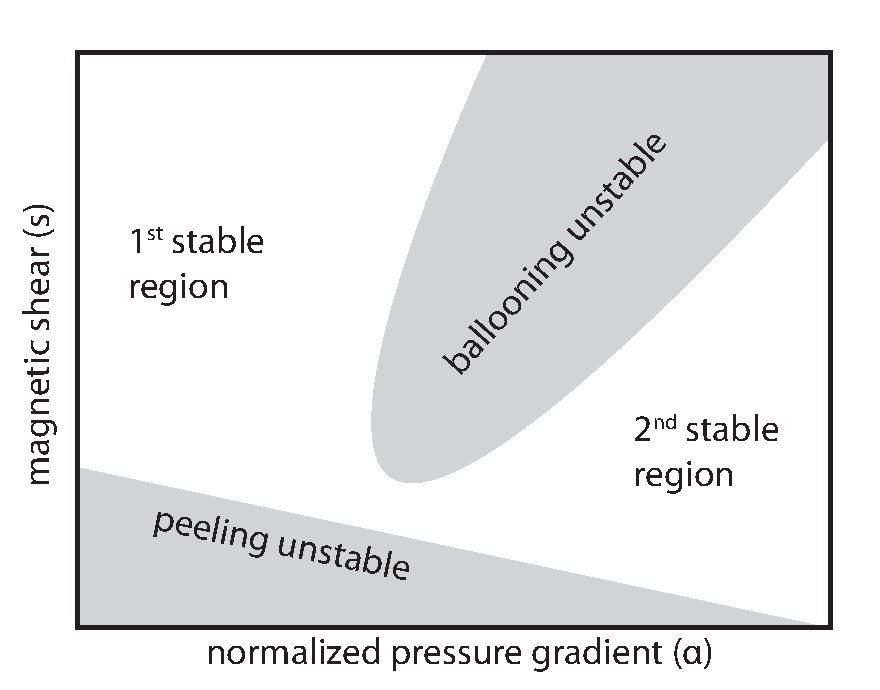
\includegraphics[width=100mm]{graphics/ModelingTheory/salpha.pdf}}
\end{figure}

However, high-$n$ peeling modes do not capture the entirety of current-driven physics in the edge.  Low-$n$ kink modes can also destabilize within the pedestal due to the strongly-peaked current density profile due to the bootstrap effect \cite{Snyder2002}.  Moreover, multiple harmonics of the edge kink mode may couple to each other at finite $n$ due to the broader radial extent of the mode, as well as coupling with pressure-driven ballooning modes due to the strong pressure gradient \cite{Wilson1999,Snyder2004}.  Unlike the $n \rightarrow \infty$ peeling and ballooning modes, each of which may be formulated with a simple one-dimensional calculation, treatment of the finite-$n$ coupled modes requires a more careful 2D treatment.

\subsection{Coupled Modes -- the ELITE Code}\label{subsec:mod_elite}

\begin{figure}
 \pushtooutside
 \fcapside[60mm]{\caption[Schematic of finite-$n$ coupled peeling-ballooning instabilities.]{Schematic in $s-\alpha_{MHD}$ space of finite-$n$ coupled peeling-ballooning instabilities, with the infinite-$n$ decoupled results (see \cref{fig:salpha}) shown by the dashed lines.  Mode coupling tends to stabilize finite-$n$ ballooning modes.  However, the coupled modes can close off access to the second-stable regime; only in cases with very strong ``magnetic wells'' (typically achieved with extreme plasma shaping) does this access reopen.}\label{fig:salpha_coupled}}{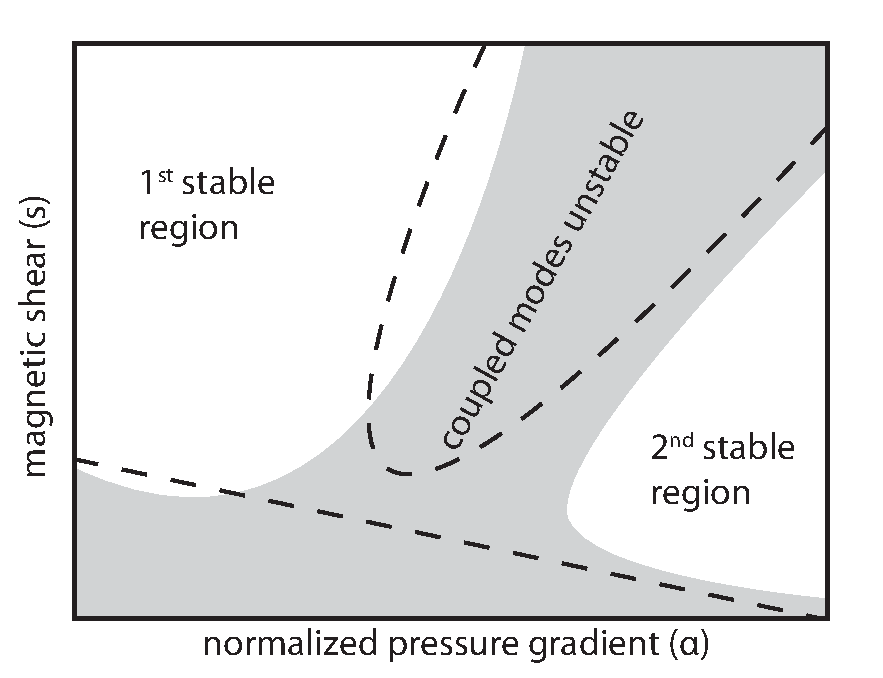
\includegraphics[width=100mm]{graphics/ModelingTheory/salpha_coupled.pdf}}
\end{figure}

The high-$n$ limits for the ballooning and peeling modes (note here that we refer to all current-driven modes in the edge as ``peeling,'' in order to distinguish them from core kink modes) yield straightforward, one-dimensional constraints on the MHD stability of the pedestal.  However, finite-larmor-radius and diamagnetic effects tend to stabilize high-$n$ modes, making this approximation relatively poor \cite{Snyder2004} -- instead, the pedestal is generally limited by finite modes with toroidal wavenumbers in the range $5 \le n \le 40$.  In this range, modes are radially broad enough that they are not cleanly localized on the corresponding rational surface, and may couple to other poloidal harmonics on nearby rational surfaces \cite{Connor1998a}.  Moreover, pressure-driven ballooning and current-driven peeling modes may couple, generating modes driven by both free-energy sources, with sufficient radial extent to affect the entire pedestal region -- driving the large, explosive crashes associated with type-I ELMs \cite{Wilson2002}.  Treatment of these modes requires a full two-dimensional approach -- we use the ``Edge-Localized Instabilities in Tokamak Equilibria'' or ELITE code \cite{Wilson1999,Wilson2002,Snyder2002} to calculate both the growth rate and eigenmode structure for these coupled modes.

ELITE utilizes the expansion of the free energy in $O(n^{-1})$ found in earlier studies of peeling and ballooning modes (see \cref{eq:dW_balloon,eq:dW_balloon_current}), with an additional boundary term for the peeling drive \cite{Wilson2002,Dowsett2014}, reproduced here for completeness:

\begin{equation}\label{eq:dW_ELITE}
 \begin{aligned}
  \delta W &= \pi \iint d\psi d\chi \Bigg\{ \frac{JB^2}{R^2 B_p^2} \left| k_\parallel X \right|^2 + \frac{R^2 B_p^2}{JB^2} \left| \frac{1}{n} \frac{\partial}{\partial \psi} \left( JB k_\parallel X \right) \right|^2\\
  &\quad- \frac{2J}{B^2} \frac{dp}{d\psi} \left[ \left| X \right|^2 \frac{\partial}{\partial \psi} \left( p + \frac{B^2}{2} \right) - \frac{iF}{JB^2} \frac{\partial}{\partial \chi} \left( \frac{B^2}{2} \right) \frac{X^*}{n} \frac{\partial X}{\partial \psi} \right]\\
  &\quad-\frac{X^*}{n} JBk_\parallel \left( \sigma' X \right) + \frac{1}{n} \left[ PJBk_\parallel^* Q^* + P^* JBk_\parallel Q \right]\\
  &\quad+ \frac{\partial}{\partial \psi} \left[ \frac{\sigma}{n} X^* JBk_\parallel X \right] \Bigg\}
 \end{aligned}
\end{equation}

\noindent with $P$, $Q$, and $\sigma$ as defined in \cref{eq:dW_current_defs}.  Given this formulation, the methodology used in ELITE is straightforward.  First, poloidal variation is encoded in a ``straight field line'' angle $\omega$ c\cite{Wilson1999},

\begin{equation}\label{eq:ELITE_angle}
 \omega = \frac{1}{q} \int^\chi \nu \;d\chi
\end{equation}

\noindent (recall that the rotational transform and safety factor $q$ are encoded such that $2\pi q = \oint \nu \;d\chi$).  Using this, the perturbation $X = RB_p \xi_\psi$ is decomposed into individual poloidal harmonics,

\begin{equation}\label{eq:ELITE_x}
 X = \sum_m u_m(\psi) e^{-im\omega}
\end{equation}

\noindent where at fixed $n$ each $u_m$ describes the eigenmodes centered on rational surfaces determined by each $(m,n)$ pair.  It can be shown \cite{Wilson2002} that this yields the relation

\begin{equation}\label{eq:ELITE_y}
 JBk_\parallel X = \sum_m \left(-\frac{\nu}{q}\right) \left(m-nq\right) u_m(x)e^{-im\omega}
\end{equation}

\noindent motivating the introduction of the radial variable $x = m_0 - nq$, where $m_0$ is the poloidal mode number of an arbitrary reference rational surface (by convention, we use the first rational surface outside the plasma, as was used in the high-$n$ peeling mode in \cref{subsec:mod_peel} \cite{Wilson2002}).  This describes spatial variation over the expected length scale for the radial extent of $u_m$, and is a straightforward conversion from $\psi$.  It is worth noting that ELITE does not treat the separatrix in its calculations, instead truncating the calculation at an internal surface (typically $99.5-99.8\%$ of poloidal flux), which prevents a singularity in $x$; although peeling modes are highly unstable at the X-point, high local collisionality prevents the omission from significantly affecting the overall result \cite{Snyder2009a}.  The Euler-Lagrange equations minimizing the potential energy may be expressed as a set of coupled second-order ordinary differential equations of the form \cite{
Dowsett2014}

\begin{equation}\label{eq:ELITE_eqs}
 A^{(2)}_{m,m'} \frac{d^2 u_m}{d\psi^2} + A^{(1)}_{m,m'} \frac{du_m}{d\psi} + A^{(0)}_{m,m'} u_m = 0
\end{equation}

\noindent where the coefficients $A$ are matrix elements describing the coupling between two modes $m$ and $m'$ (see Wilson \etal \cite{Wilson2002} for definitions).  Efficient computation of these eigenmodes is assisted by two simplifications: first, while the eigenmodes $u_m$ vary on a very short length scale $x$, comparable to the spacing between rational surfaces, the equilibrium parameters used in the calculation of the matrix elements $A$ vary more slowly, and can be calculated on a coarser mesh than that needed to evaluate \cref{eq:ELITE_eqs}.  Second, this radial localization of $u_m$ means that only harmonics on nearby rational surfaces will strongly couple -- other modes can be ignored in the computation to save time \cite{Wilson2002}.  An example of the eigenmode structure for an $n=30$ ballooning mode is shown in \cref{fig:pb_modestructure}, with the poloidal variation of the displacement amplitude (strongest at the outboard midplane, as is typical for ballooning modes) shown at left and the 
radial structure of the modes shown at right.

\begin{figure}[t]
 \pushtooutside
 \ffigbox[\FBwidth]{\includegraphics[width=150mm]{graphics/ModelingTheory/pb_modestructure.pdf}}{\caption[Mode structure for $n=30$ model calculated by ELITE.]{Mode structure for an $n=30$ ballooning mode calculated by ELITE.  (left) Contour plot of radial perturbations from the mode.  The mode is edge-localized and strongest at the outboard midplane, consistent with an edge ballooning mode.  (right) Eigenmode structure of the $n=30$ mode.  Each peak is a poloidal harmonic localized around the rational flux surface determined by the corresponding poloidal mode number $m$ for $n=30$.  The mode is strongest in the steep gradient region, but extends inward due to the comparatively high mode number (eigenmode envelope encompasses $O(n^{1/3})$ flux surfaces).  Note that, as ELITE cannot treat the separatrix, the mode calculation truncates at $\psi_{norm} = 0.995$.}\label{fig:pb_modestructure}}
\end{figure}

\begin{itemize}
 \item EDA H-mode modeled to be ideal-ballooning stable; P-B only describes ELMy H-mode \cite{Mossessian2002}
 \item DIII-D VH-modes terminate in giant p-b driven ELM \cite{Turnbull2003}
 \item strong shaping impacts stability contour in $j-\alpha_{MHD}$ space \cite{Snyder2009}
 \item collisionality $\rightarrow$ bootstrap current $\rightarrow$ magnetic shear in edge sets where in stability contour pedestal hits \cite{Snyder2009}
 \item due to interplay, nonlocal effects between shaping, collisionality, rotation, shafranov shift, safety factor, must calculate P-B stability in 2D: can't reduce to scalar parametrization \cite{Snyder2009}
 \item Snyder2009 refs Huysmans2005, Turnbull2003, Medvedev2006 \cite{Huysmans2005,Turnbull2003,Medvedev2006} for reviews of alternate MHD codes
 \item alternate MHD codes: GATO \cite{Bernard1981}, MISHKA \cite{Huysmans2001,Mikhailovskii1997}, KINX \cite{Degtyarev1997,Medvedev2006}, MARG2D \cite{Aiba2006,Aiba2007}
 \item RMP approaches P-B boundary, EDA, type-III ELMs P-B stable, grassy/type-II ELMs near boundary, QH near low-$n$ peeling side -- P-B boundary figure of merit in general for H-mode pedestal \cite{Snyder2009}.  RMP calcs stable, goes ELMing and crosses boundary as soon as coils are turned off \cite{Snyder2009a}
 \item very low $n$ ($n < 3$) modes omitted from ELITE: low-$n$ edge modes rarely more unstable than $n \sim 5$, code cannot distinguish from core kink modes, low-$n$ modes stabilized by interaction with wall \cite{Snyder2009}
 \item ELITE omits X-point from calculation due to required extremely high RZ point density; peeling modes highly unstable there, but high collisionality at LCFS suppresses.  Calculation usually truncated at 99.8\% flux \cite{Snyder2009a}
 \item check Snyder2009a for ELITE alternate refs; Huysmans2005, Wilson2006 for reviews \cite{Snyder2009a,Huysmans2005,Wilson2006}
\end{itemize}

\begin{figure}
 \pushtooutside
 \fcapside[60mm]{\caption[Schematic of peeling-ballooning MHD stability space.]{Schematic of the stability space to coupled peeling-ballooning MHD modes, set by the edge pressure gradient and current density.  Ballooning modes are driven by pressure gradient but stabilized by magnetic shear driven by edge currents, while kink/peeling modes are current-driven but stabilized by pressure gradients.  \note{Ref to Snyder?}}\label{fig:mod_pbcartoon}}{\includegraphics[width=100mm]{graphics/ModelingTheory/pbcartoon.pdf}}
\end{figure}

% move this to ch 4!
% \begin{figure}
%  \pushtooutside
%  \fcapside[60mm]{\caption[ELITE calculation of P-B stability in a C-Mod ELMy H-mode.]{Calculation of the peeling-ballooning MHD stability contour from ELITE for an ELMy H-mode pedestal on C-Mod.  To within error bars, the pedestal lies on the peeling-ballooning boundary.  The comparatively higher collisionality typical of C-Mod H-mode pedestals pushes the MHD behavior of the pedestal towards higher-$n$, pure-ballooning modes, although moderate-$n$ coupled modes in the ``nose'' of the stability contour are also common.}\label{fig:mod_elmy_elite}}{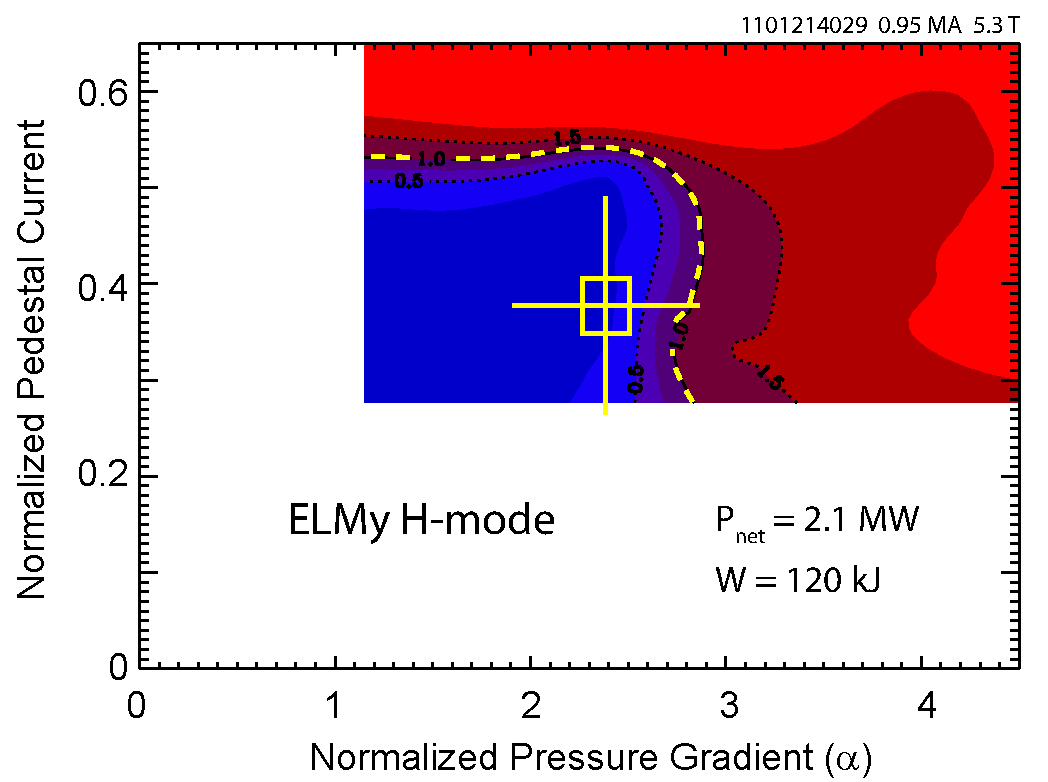
\includegraphics[width=100mm]{graphics/ModelingTheory/elmy_elite_nobal.pdf}}
% \end{figure}

\nicesectionending

\section{Kinetic-Ballooning Turbulence Modeling}\label{sec:mod_turbulence}

Following the L-H transition, the $\vec{E}\times\vec{B}$ flows associated with the formation of the pedestal and transition to high confinement should continue to rise, due to the strong increase in the diamagnetic term due to the pedestal \cite{Snyder2009}.  However, the pedestal gradient appears to be limited, even before the onset of an ELM -- thus, there must be a mechanism limiting the pedestal prior to the onset of the ideal MHD instability (\cref{sec:mod_pb}).  As the $\vec{E}\times\vec{B}$ flow strongly suppresses long-wavelength turbulence, short-wavelength turbulent modes appear to be an ideal candidate.  Electron-temperature-gradient (ETG) modes at short wavelengths is more likely to modify the interplay between density and temperature in the pedestal \cite{Snyder2009} -- instead, the recent efforts have focused on the kinetic-ballooning mode (KBM) for a constraint on the pressure pedestal.

The KBM arises from the introduction of kinetic effects in an extension of the high-$n$ ideal ballooning MHD formalism, introduced in \cref{subsec:mod_balloon} \cite{Tang1980}.  Although the initial assumptions for each are quite different -- the ideal MHD energy principle (\cref{eq:dW_balloon}) requires high collisionality for the coupled fluid treatment, the kinetic-energy formulation treating a collisionless plasma with trapped-particle effects results in a very similar fluid-like relation \cite{Tang1980}.  Earlier gyrokinetic studies focused on electrostatic fluctuations, of which the ion-temperature gradient (ITG) mode is dominant; however, the introduction of magnetic fluctuations both modifies ITG dynamics, and allows for the formation of the electromagnetic KBM fluctuation \cite{Snyder2001}.  In regimes with high $\beta$ or steep pressure gradients -- in short, exactly the plasmas of concern for high-performance regimes -- electrostatic simplifications to gyrokinetic turbulence break down, necessitating treatment of the KBM in modeling \cite{Snyder1999,Snyder2001}.

Gyrokinetic and gyrofluid simulations using the necessary electromagnetic treatment \cite{Jenko2001,Snyder2001,Scott2003,Candy2005} found the onset of a distinct turbulent mode at high beta, overtaking the usually-dominant ITG and trapped-electron mode (TEM) turbulence at low and moderate beta, respectively.  Above this threshold in $\beta$ (more properly, a threshold in $\alpha_{MHD}$), simulations using the GYRO code \cite{Candy2003} found that the mode onset was highly stiff -- that is, the growth rate of the mode increases extremely quickly even in plasmas just above the onset threshold \cite{Candy2005} -- and is insensitive to $\vec{E}\times\vec{B}$ shear, such that the mode drives transport levels sufficient to constrain the pedestal gradient near the critical $\alpha_{MHD}$ \cite{Snyder2009}.  Moreover, gyrofluid simulations found that the KBM is destabilized near the infinite-$n$ ideal ballooning limit -- in cases with a flat temperature profile, the onset is precisely matched to the calculated MHD limit, while the inclusion of a finite temperature gradient somewhat reduced the onset $\alpha_{MHD}$ due to ion drift resonance effects \cite{Snyder2001}.  This motivates the use of more straightforward high-$n$ MHD calculations (see \cref{subsec:mod_balloon}) to calculate the KBM threshold for the purposes of this thesis, rather than complex gyrokinetic/gyrofluid simulations.

The stiff onset of the kinetic-ballooning mode, and accompanying limits to the pedestal pressure gradient, allows for a heuristic scaling for the pedestal width \cite{Snyder2009}.  To good approximation, the critical gradient is simply given by $\alpha_c \sim \beta_{p,ped}/\Delta$ for the poloidal beta at the pedestal top and the pedestal width $\Delta$ expressed in (normalized) poloidal flux -- thus we require $\Delta \sim \beta_{p,ped}/\alpha_c$.  As with ideal MHD ballooning modes, the KBM is sensitive to magnetic shear.  However, at the outboard midplane (where magnetic curvature is least favorable) the local shear is such that the critical $\alpha_c$ increases with decreasing shear, $\alpha_c \sim 1/s^{1/2}$.  In the pedestal, we expect the shear to trend as $1/\langle j \rangle$, which to lowest-order approximation is simply $1/\beta_{p,ped}$ as the current in the pedestal is bootstrap-dominated\gnote{not sure I follow phil's reasoning here}.  This implies $\alpha_c \sim \beta_{p,ped}^{1/2}$ and therefore $\Delta \sim \beta_{p,ped}^{1/2}$.  This trend is in accordance with experimental observations on DIII-D \cite{Osborne1998}, JT-60U \cite{Oyama2005,Urano2008}, ASDEX Upgrade \cite{Gruber1999,Beurskens2011} and Alcator C-Mod \cite{LaBombard2008}.  Moreover, the growth of the pedestal between ELMs appears to maintain a limited pressure gradient \cite{Maggi2010,Hughes2013}, and pedestal fluctuations saturate early in the ELM cycle \cite{Diallo2014}, consistent with the idea that KBM turbulence constrains the pedestal indepedent of explosive ELM-driven transport.

\subsection{The Ballooning-Critical Pedestal Technique}\label{subsec:mod_bcp}

The arguments detailed above lead to an intuitive expression for the pedestal width and height based on KBM limits, $\Delta \sim \beta_{p,ped}^{1/2}$.  However, full quantification of the KBM constraint from first principles requires a more detailed treatment.  The analogous onset of the KBM to the infinite-$n$ ideal ballooning MHD mode allows a computationally-efficient approach to the turbulence threshold.

The KBM is an approximately local effect due to its short scale length -- as such, no single calculated mode can describe the destabilization of the entire pedestal without a highly involved nonlocal calculation of the stability across the pedestal profile.  A far more efficient and straightforward model can be developed using the ``ballooning critical pedestal'' (BCP) technique \cite{Snyder2010,Snyder2011}, which finds the point where half of the pedestal is locally at or beyond criticality for the KBM.  At fixed pedestal width, the height is incremented to increase the pressure gradient, following the same approach as the peeling-ballooning calculation.  At each increment, the stability of the pedestal to high-$n$ ideal ballooning MHD modes is calculated, \eg using the BALOO code \cite{Connor1979,Miller1987}.  As the infinite-$n$ modes calculated by BALOO are also perfectly localized on the corresponding rational flux surfaces, the code finds unstable surfaces in the pedestal region and the width of the pedestal covered by these surfaces.  When half of the pedestal width is thus unstable, the KBM threshold is said to have been reached.  This approach is highly numerically efficient -- as the ballooning MHD criterion reduces in the infinite-$n$ limit to a straightforward one-dimensional eigenvalue problem \cite{Connor1979} that can be computed efficiently -- and fairly robust, although it does require the unstable region of the pedestal to be well-defined and bounded (typically the ``middle half'' of the pedestal, where the pressure gradient is steepest).  This assumption can break down at very strong shaping or low aspect ratio \cite{Snyder2011}.\nicesectionending

\section{The EPED Model}\label{sec:mod_eped}

In light of the importance of the pedestal structure for optimized fusion performance -- both by maximizing fusion power density via the pressure pedestal height constraint on core profiles \cite{Kinsey2011}, and by avoiding or mitigating large, damaging ELMs \cite{Loarte2003,Federici2003} -- a predictive understanding of the pedestal is highly desirable for planned operations on ITER and beyond.  Models based on peeling-ballooning MHD instability, particularly the ELITE code (\cref{subsec:mod_elite}), have proven quite successful at capturing the limiting physics of the ELMy H-mode pedestal.  However, these calculations typically rely on experimental profiles and magnetic equilibria reconstructed after the fact, and as such cannot by themselves provide predictive capability.  Similarly, the constraint set by kinetic-ballooning mode (KBM) turbulence (\cref{sec:mod_turbulence}) corresponds well with pedestal observations in profiles with steep pressure gradients in the pedestal, but cannot by itself uniquely constrain the pedestal structure.  Here we introduce the EPED series of models \cite{Snyder2011}, which combines these two constraints into a single predictive model for the ELMy H-mode pedestal.

To incorporate predictive capability into the peeling-ballooning MHD stability model calculated by ELITE, the EPED model must characterize peeling-ballooning stability as accurately as possible using only parameters known prior to the plasma discharge, set by operator control; however, as discussed in \cref{subsec:mod_elite}, the inherent nonlocality of the problem still requires a 2-dimensional MHD calculation.  To that end, the model employs a set of model Miller equilibria \cite{Miller1998}, up/down-symmetric equilibria allowing for plasma elongation and triangularity defined with analytic plasma profiles such that the essential physics in the pedestal (namely, the pressure gradient and bootstrap current profiles) is nearly matched to experimental conditions \cite{Snyder2009}.  Using this setup, the model equilibria may be defined by a small set of scalar parameters for use in ELITE: major and minor radius $R$ and $a$, elongation and shaping $\kappa$, $\delta$ (recall that in these up/down-symmetric equilibria $\delta_l = \delta_u = \delta$), plasma current $I_p$, and applied field $B_T$, set the magnetic equilibrium when combined with the target global normalized pressure (typically the Troyon normalized $\beta_N$ \cite{Troyon1984}).  Global beta also impacts the pedestal stability via the beneficial effect of increased Shafranov shift in the core on MHD stability\gnote{ref this in peeling-ballooning section!}.  The model additionally takes as inputs the density at the pedestal top $n_{e,ped}$ and the pedestal width $\Delta$ in normalized poloidal flux (note that the density and temperature profiles are defined to have the same width) to constrain the pressure and current profiles, with the current calculated from the density and temperature profiles from the analytic Sauter formula, \cref{eq:jboot} \cite{Sauter1999}.

The calculation of the peeling-ballooning stability boundary is straightforward -- at a fixed pedestal width, the pressure pedestal height (and, accordingly, the MHD instability drives from the edge pressure gradient and current density) is increased in increments until the stability boundary is reached \cite{Snyder2009}.  The interdependence between pedestal width and height is determined by repeating the calculation at a range of pedestal widths, determining a relation between the pressure pedestal width and height for a given model equilibrium.  To lowest order, the MHD limit is a limit on $\nabla p$, leading one to expect a linear relation between the pedestal width and height.  However, nonlocal effects on the MHD stability -- in particular, the broader, lower-$n$ modes destabilized by wider pedestals leading to reduced maximum $\alpha_{MHD}$ at wider $\Delta$ -- reduces the linear dependence, leading to a rough scaling of $p_{ped} \sim \Delta^{3/4}$ set by the peeling-ballooning stability boundary \cite{Snyder2009a}.

On its own, the peeling-ballooning MHD constraint defines the pedestal height as a function of width, necessitating a second constraint to allow a unique predictive solution.  The Kinetic Ballooning Mode (KBM), described in \cref{sec:mod_turbulence}, limits the pedestal gradient with a relation $p_{ped} \sim \Delta^2$ (more precisely, $\Delta \sim \beta_{p,ped}^{1/2}$).  This constraint is sufficiently distinct from that enforced by peeling-ballooning MHD  that only a single nontrivial solution satisfying both exists -- thereby uniquely predicting the pedestal width and height.  An example of the prediction at the intersection of the P-B and KBM constraints, along with the corresponding experimental result \cite{Snyder2011}, is shown in \cref{fig:mod_epedcartoon}.

\begin{figure}[ht]
 \pushtooutside
 \fcapside[60mm]{\caption[Illustration of the peeling-ballooning MHD and KBM constraints used in the EPED model.]{Illustration of the peeling-ballooning MHD and kinetic-ballooning turbulent constraints used in the EPED model.  The peeling-ballooning constraint, calculated by ELITE, results in a trend roughly of $p_{ped} \sim \Delta_\psi^{3/4}$, while the KBM width constraint calculated via the ballooning-critical pedestal (BCP) technique sets $p_{ped} \sim \Delta_\psi^{2}$.  The unique solution to these constraints is the EPED prediction for the pedestal width and height.  The prediction is here shown compared to the measured pedestal from DIII-D shot 132003 (reproduced from \cite{Snyder2011}) \note{get permission}}\label{fig:mod_epedcartoon}}{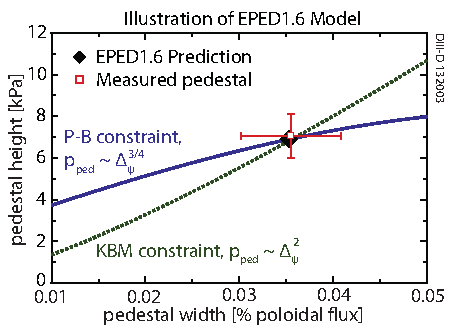
\includegraphics[width=100mm]{graphics/ModelingTheory/epedcartoon.pdf}}
\end{figure}

\subsection{EPED1}\label{subsec:mod_eped1}

The simplest version of the EPED series, EPED1 \cite{Snyder2009}, takes advantage of the dominant scaling of the width with $\beta_{p,ped}$ in the KBM constraint: as little secondary variation of the width beyond $\Delta \sim \beta_{p,ped}^{1/2}$ is seen with other expected controlling parameters, \eg $\nu^*$, $\rho^*$ or $\rho^*_{pol}$, $n_{e,ped}$ \cite{Snyder2009} (\cf \cref{sec:mod_early}, particularly \cref{subsec:mod_ionorbitloss}), the constraint is reduced to a single relation $\Delta = c \beta_{p,ped}^{1/2}$ with a fitted value for $c$.  For historical reasons based on DIII-D data, EPED1 uses $c = 0.076$, although a newer multi-machine fit produces $c = 0.084$ \cite{Snyder2011}. 

To calculate the threshold for the peeling-ballooning MHD instability, the growth rate as calculated by ELITE must be balanced against against the inherent stabilizing effect of plasma diamagnetism in the pedestal\gnote{ref or elaboration on this, or mention in ELITE section?}.  In the EPED1 model this effect is taken to be the solution to $\gamma_{MHD} = \omega (\omega - \omega_{*pi})$, where $\gamma_{MHD}$ is the instability growth rate and $\omega_{*pi}$ is the half-maximum diamagnetic frequency in the pedestal \cite{Snyder2009}.  This leads to a threshold for the growth rate of $\gamma_{MHD} > \omega_{*pi}/2$ for the peeling-ballooning onset\gnote{refs are remarkably reticent to define $\omega_{*pi}$}.  Despite this simple treatment of the KBM and P-B constraints, the EPED1 model is capable of producing predictions with a systematic $\pm 15-20\%$ uncertainty across a range of parameters \cite{Snyder2009,Snyder2010}.

\subsection{EPED1.6}\label{subsec:mod_eped16}

Although the bulk of the variation in the KBM-constrained pedestal width is captured by the $\beta_{p,ped}$ scaling, it is nevertheless desirable to account for its effects on the scale factor of the trend -- more properly, the weakly-varying function $G(\nu^*,\varepsilon,...)$ such that $\Delta = G \beta_{p,ped}^{1/2}$ -- allowing EPED to make first-principles predictions (in that the constraint is not dependent on a scale factor set by fitted data).  

The EPED1.6 implementation \cite{Snyder2010,Snyder2011} achieves this by directly calculating the KBM constraint via the ``ballooning critical pedestal'' (BCP) technique, described in \cref{subsec:mod_bcp}.    By performing this calculation across a range of pedestal widths and fitting the result against $\beta_{p,ped}$, a first-principles calculation of the KBM pedestal constraint is generated and paired with the peeling-ballooning MHD result \cite{Snyder2011}.  While this approach is more computationally expensive than the fixed scaling used in EPED1, the BCP calculation allows the effects of collisionality and shaping on the KBM threshold to be properly accounted for -- this manifests in a range of scale factors, $\langle G \rangle \approx 0.07-0.1$, that are comparable to the fitted result used in EPED1, but are specific to discharge characteristics.

The simple diamagnetic stabilization model used in EPED1, $\gamma_{MHD} > \omega_{*pi}/2$, also fails to capture important physics in the pedestal -- the model assumes a constant diamagnetic frequency $\omega_{*pi}$ for the stabilization of the peeling-ballooning modes, while in fact the diamagnetic frequency varies rapidly over the pedestal \cite{Snyder2010}.  EPED1.6 replaces this with an ``effective'' diamagnetic frequency $\omega_{*eff}$, determined by directly calculating the diamagnetic stabilization of peeling-ballooning modes in the fluid code BOUT++ \cite{Xu2010,Xia2013}.  This provides stronger stabilization of higher-$n$ ($n > \sim 12$) modes at higher collisionality than that found in the simple linear model \cite{Snyder2011,Hughes2013}, a correction that is particularly necessary for the comparatively high-collisionality pedestals in ELMy H-modes on C-Mod \cite{Hughes2013}.

\subsection{EPED Model Implementation \& ITER Predictions}\label{subsec:mod_eped_iter}

The EPED model has been extensively tested on numerous machines, particularly on DIII-D \cite{Snyder2011,Groebner2013}, JT-60U \cite{Snyder2009a}, C-Mod \cite{Walk2012}, and KSTAR \cite{Han2013}.  The model has also been tested on NSTX \cite{Groebner2013}, with limited success due to breakdown of the assumptions inherent to the KBM constraint at small aspect ratio \cite{Snyder2009a}.  Given the proximity of the pedestal to the peeling-ballooning MHD and KBM turbulence limits in most high-performance regimes, it is expected that EPED predictions are viable as a figure of merit for H-mode operation on ITER \cite{Snyder2011,Snyder2012}.

\begin{figure}[ht]
 \pushtooutside
 \fcapside[60mm]{\caption[EPED predictions versus measured pressure pedestal heights.]{EPED predictions versus measured pressure pedestal heights from DIII-D and C-Mod, spanning a significant range of pedestal pressures.  Notably, C-Mod pressure pedestals reach within a factor of $\sim 2$ of the predicted ITER pedestal height.  Reproduced from \cite{Hughes2013} \note{permission!}}\label{fig:mod_epedpredictions}}{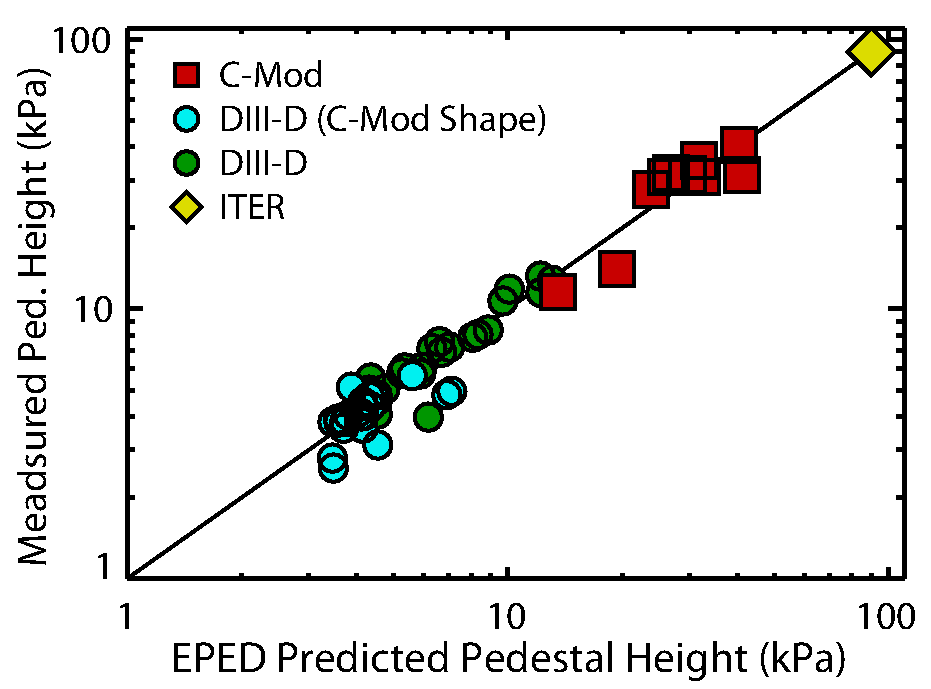
\includegraphics[width=100mm]{graphics/ModelingTheory/eped.pdf}}
\end{figure}

\noindent Notably, EPED predictions for ITER (shown compared to results from DIII-D and C-Mod \cite{Hughes2013} in \cref{fig:mod_epedpredictions}) predict pedestal pressures of $\beta_{N,ped} \sim 0.6-0.7$, corresponding to $p_{ped} \sim \SI{90}{\kilo\pascal}$, at a pedestal width of $\Delta \sim 4\%$ \cite{Snyder2009a,Snyder2011}.  This is within a factor of $\sim 2-3$ of the range of experimental results on which EPED has been tested \cite{Walk2012,Hughes2013}, and is consistent with the planned $Q=10$ operation on ITER assuming sufficient optimization of core and pedestal profiles \cite{Snyder2011,Snyder2012}.  Although development is ongoing for the EPED model series, it has demonstrated viable predictive capability for H-mode pedestals in a variety of conditions for conventional-aspect-ratio tokamaks.\nicechapterending

\bibliographystyle{../plainurl}
\bibliography{../references}